\documentclass[man, fleqn, noextraspace]{apa6}

\usepackage{amssymb,amsmath}
\usepackage{ifxetex,ifluatex}
\usepackage{fixltx2e} % provides \textsubscript
\ifnum 0\ifxetex 1\fi\ifluatex 1\fi=0 % if pdftex
  \usepackage[T1]{fontenc}
  \usepackage[utf8]{inputenc}
\else % if luatex or xelatex
  \ifxetex
    \usepackage{mathspec}
    \usepackage{xltxtra,xunicode}
  \else
    \usepackage{fontspec}
  \fi
  \defaultfontfeatures{Mapping=tex-text,Scale=MatchLowercase}
  \newcommand{\euro}{€}
\fi
% use upquote if available, for straight quotes in verbatim environments
\IfFileExists{upquote.sty}{\usepackage{upquote}}{}
% use microtype if available
\IfFileExists{microtype.sty}{\usepackage{microtype}}{}

% Table formatting
\usepackage{longtable, booktabs}
\usepackage{lscape}
% \usepackage[counterclockwise]{rotating}   % Landscape page setup for large tables
\usepackage{multirow}		% Table styling
\usepackage{tabularx}		% Control Column width
\usepackage[flushleft]{threeparttable}	% Allows for three part tables with a specified notes section
\usepackage{threeparttablex}            % Lets threeparttable work with longtable

% Create new environments so endfloat can handle them
% \newenvironment{ltable}
%   {\begin{landscape}\begin{center}\begin{threeparttable}}
%   {\end{threeparttable}\end{center}\end{landscape}}

\newenvironment{lltable}
  {\begin{landscape}\begin{center}\begin{ThreePartTable}}
  {\end{ThreePartTable}\end{center}\end{landscape}}

  \usepackage{ifthen} % Only add declarations when endfloat package is loaded
  \ifthenelse{\equal{\string man, fleqn, noextraspace}{\string man}}{%
   \DeclareDelayedFloatFlavor{ThreePartTable}{table} % Make endfloat play with longtable
   % \DeclareDelayedFloatFlavor{ltable}{table} % Make endfloat play with lscape
   \DeclareDelayedFloatFlavor{lltable}{table} % Make endfloat play with lscape & longtable
  }{}%



% The following enables adjusting longtable caption width to table width
% Solution found at http://golatex.de/longtable-mit-caption-so-breit-wie-die-tabelle-t15767.html
\makeatletter
\newcommand\LastLTentrywidth{1em}
\newlength\longtablewidth
\setlength{\longtablewidth}{1in}
\newcommand\getlongtablewidth{%
 \begingroup
  \ifcsname LT@\roman{LT@tables}\endcsname
  \global\longtablewidth=0pt
  \renewcommand\LT@entry[2]{\global\advance\longtablewidth by ##2\relax\gdef\LastLTentrywidth{##2}}%
  \@nameuse{LT@\roman{LT@tables}}%
  \fi
\endgroup}


  \usepackage{graphicx}
  \makeatletter
  \def\maxwidth{\ifdim\Gin@nat@width>\linewidth\linewidth\else\Gin@nat@width\fi}
  \def\maxheight{\ifdim\Gin@nat@height>\textheight\textheight\else\Gin@nat@height\fi}
  \makeatother
  % Scale images if necessary, so that they will not overflow the page
  % margins by default, and it is still possible to overwrite the defaults
  % using explicit options in \includegraphics[width, height, ...]{}
  \setkeys{Gin}{width=\maxwidth,height=\maxheight,keepaspectratio}
\ifxetex
  \usepackage[setpagesize=false, % page size defined by xetex
              unicode=false, % unicode breaks when used with xetex
              xetex]{hyperref}
\else
  \usepackage[unicode=true]{hyperref}
\fi
\hypersetup{breaklinks=true,
            pdfauthor={},
            pdftitle={Exploring and Visualizing School Achievement and School Effects},
            colorlinks=true,
            citecolor=blue,
            urlcolor=blue,
            linkcolor=black,
            pdfborder={0 0 0}}
\urlstyle{same}  % don't use monospace font for urls

\setlength{\parindent}{0pt}
%\setlength{\parskip}{0pt plus 0pt minus 0pt}

\setlength{\emergencystretch}{3em}  % prevent overfull lines


% Manuscript styling
\captionsetup{font=singlespacing,justification=justified}
\usepackage{csquotes}
\usepackage{upgreek}



\usepackage{tikz} % Variable definition to generate author note

% fix for \tightlist problem in pandoc 1.14
\providecommand{\tightlist}{%
  \setlength{\itemsep}{0pt}\setlength{\parskip}{0pt}}

% Essential manuscript parts
  \title{Exploring and Visualizing School Achievement and School Effects}

  \shorttitle{Visualizing School Achievement}


  \author{Daniel Anderson\textsuperscript{1}~\& Joseph Stevens\textsuperscript{1}}

  % \def\affdep{{"", ""}}%
  % \def\affcity{{"", ""}}%

  \affiliation{
    \vspace{0.5cm}
          \textsuperscript{1} University of Oregon  }

  \authornote{
    The research reported here was supported by the Institute of Education
    Sciences, U.S. Department of Education, through Grant R324C110004,
    awarded to the University of Oregon. The opinions expressed are those of
    the authors and do not represent views of the Institute or the U.S.
    Department of Education.
    
    Correspondence concerning this article should be addressed to Daniel
    Anderson, 5262 University of Oregon. E-mail:
    \href{mailto:daniela@uoregon.edu}{\nolinkurl{daniela@uoregon.edu}}
  }


  \abstract{Recent years have seen a push for more open data as a means of
facilitating transparency and opening doors for further research. Since
the implementation of the No Child Left Behind Act, schools and
districts across the country have been required to publicly report the
number of students scoring in each performance level classification on
the statewide test, disaggregated by student subgroups (e.g., gender,
race/ethnicity). These data represent a ``coarsening'' of the underlying
continuous data by binning the distributions into categories. The
purpose of this paper is to evaluate the extent to which achievement gap
estimates from student-level data align with those estimates from
coarsened data, using the approach suggested by Ho and Reardon (2012).
Following the evaluation, we use this approach to visualize differences
in school-level achievement gaps using publicly-available data, and
visualize these estimates through geo-spatial mapping. We overlay
demographic data as a means to visually evaluate the extent to which
demographics of the surrounding area correspond to school-level
achievement gaps.}
  \keywords{Effect Size, Achievement Gaps, Visualization, Maps \\

    \indent Word count: X
  }




  \raggedbottom

\usepackage{amsthm}
\newtheorem{theorem}{Theorem}[section]
\newtheorem{lemma}{Lemma}[section]
\theoremstyle{definition}
\newtheorem{definition}{Definition}[section]
\newtheorem{corollary}{Corollary}[section]
\newtheorem{proposition}{Proposition}[section]
\theoremstyle{definition}
\newtheorem{example}{Example}[section]
\theoremstyle{definition}
\newtheorem{exercise}{Exercise}[section]
\theoremstyle{remark}
\newtheorem*{remark}{Remark}
\newtheorem*{solution}{Solution}
\begin{document}

\maketitle

\setcounter{secnumdepth}{0}



Recent years have seen increased attention on open data (i.e., free and
publicly available) as one component of open science (e.g., see Dawes,
Vidiasova, \& Parkhimovich, 2016; Sieber \& Johnson, 2015; Zuiderwijk \&
Janssen, 2014). The National Institute of Health (NIH), for example,
recently made 64 data sharing repositories publicly available (Kittrie
\& Chattopadhyay, 2016). The National Science Foundation (NSF) has
placed a similarly high emphasis on making data from funded projects
publicly available, as part of their Open Government Plan (National
Science Foundation, 2016). The Institute of Education Sciences (IES) has
similarly moved towards greater requirements for data sharing, with Goal
4 Effectiveness grants requiring a data sharing component since 2013,
and Goal 3 Efficacy and Replication awards requiring data sharing since
2016 (Institute of Education Sciences, 2016). Despite these movements,
data that are fully open remain rare, particularly in educational
research. For example, the website data.gov represents the \enquote{home
of the U.S. Government's open data}, housing nearly a quarter of a
million datasets. Of these datasets, only 365 were tagged with the
keyword \enquote{Education} (as of this writing), and the vast majority
of these receive an openness score of one star out of a possible five.

Privacy issues abound in educational research, given that the research
population generally includes minors. Privacy concerns may therefore
explain part of the lack of data sharing (although it should be noted
that health care and medical research often face similar privacy
concerns). One method of avoiding potential issues of confidentiality is
to first aggregate the data in some capacity, before releasing the data
publicly. This was the approach taken by the \emph{No Child Left Behind
Act} (No Child Left Behind, 2002), with data reported at the overall
school and district levels, but not at the individual student level.
NCLB required annual testing in reading and mathematics in each of
grades 3-8, and once in high school, with the results reported at the
aggregate levels by student subgroups (e.g., gender, race/ethnicity).
Cut scores were required to be established, delineating students into
various performance level classifications (PLCs). The state of
California, for example, included the following four categories in order
of increasing competency: \enquote{Not Met}, \enquote{Nearly Met},
\enquote{Met}, and \enquote{Exceeds}. The proportion of students scoring
in each of these categories, by subgroup, were also required to be
reported at each of the school and district levels by NCLB, provided a
sufficient number of students were represented within each subgroup such
that individual students could not be identified.

\hypertarget{evaluating-achievement-gaps-with-open-data}{%
\subsection{Evaluating Achievement Gaps With Open
Data}\label{evaluating-achievement-gaps-with-open-data}}

Aggregating the data to higher levels, combined with reporting test
score data by PLC proportions, helps avoid privacy concerns and allows
the data to be reported publicly. Despite mandates from NCLB on public
reporting, however, the openness of these data vary by state, in terms
of accessing the data for research purposes. Some (e.g., Oregon,
California) make the process easy, with downloadable comma separated
value (CSV) including the proportion of students scoring in each PLC for
all schools and/or districts in the state, by student subgroups. Other
states make it relatively easy to access the data for an individual
school or district (as mandated by NCLB) but rather difficult to access
across schools or districts. Further, the utility of these data for
research purposes is not particularly straightforward. While raw
percentages scoring within specific PLCs can be compared between schools
or between student subgroups, rthese differences are highly dependent
upon the placement of the cut scores (Ho, 2008, Holland (2002)).

Ideally, a transformation could be applied to the \enquote{coarsened}
data (continuous test score distributions binned into a set of ordinal
categories; Reardon \& Ho, 2015) to recover the parameters of the full
distribution for each subgroup, making the placement of the cut scores
inconsequential to evaluating subgroup differences. Ho and Reardon
(2012) and Reardon and Ho (2015) propose such an approach, in which the
coarsened data are used to construct empirical cumulative distribution
functions (ECDFs) for each group. Paired ECDFs for any two groups are
then evaluated in the form of a probability-probability (PP) plot, and
the area under the PP curve (AUC) provides an estimate of the
probability that a randomly selected students from the reference
distribution (plotted along the x-axis) would score higher than a
randomly selected student from the focal distribution (plotted along the
y-axis; see Ho \& Reardon, 2012). This proportion can then be
transformed into standard-deviation units, using the following formula,
as outlined by Ho (2009) \begin{equation}
V = \sqrt(2)\Phi^{-1}(AUC)
\end{equation} Where \(\Phi^{-1}\) represents the inverse normal
distribution. Under the assumption of respective normality, \(V\) is
equivalent to Cohen's \(D\), and the dependence upon cut scores is
removed, given that it is an estimate of difference between the paired
distributions, rather than the difference between proportions at any
particular point on the distribution. Importantly, because \(V\) can be
estimated from coarsened data, it can be used to estimate the overall
achievement gap between student subgroups using NCLB mandatorily
reported data.

\hypertarget{achievement-gaps-in-context}{%
\subsection{Achievement Gaps in
Context}\label{achievement-gaps-in-context}}

A wealth of previous research has examined achievement differences
between student subgroups. Sirin (2005), for example, conducted a
meta-analytic review of the relation between socioeconomic status (SES)
and academic achievement. The author found that, while there was a
medium to strong overall relation, the magnitude was dependent upon
(among other factors) the physical location of the school. This is
perhaps unsurprising , given that schools draw students from the
surrounding neighborhoods, and any disparities between neighborhoods
would naturally flow into disparities between schools. When evaluating
achievement gaps, it makes sense to consider characteristics of both the
school and the surrounding neighborhood/community. For example, it is
possible that the racial/ethnic makeup of the surrounding area would
relate to achievement gaps at the school, given that identifying as
Black in a school with students predominately identifying as White is
very different from identifying as Black in a school where students
predominately identify as Black (Hanushek, Kain, \& Rivkin, 2009).

In addition to school compositional effects, there is a considerable
evidence that crime rates in the surrounding area relate to student
achievement (e.g., Gonzales, Cauce, Friedman, \& Mason, 1996; McCoy,
Roy, \& Sirkman, 2013). In particular, N. K. Bowen and Bowen (1999)
found that measures of neighborhood danger were predictive of a number
of outcomes, but particularly measures of behavior and attendance. The
authors found that males and students identifying as African American
reported higher rates of exposure to both neighborhood and school
danger. These results are particularly relevant for achievement gaps
when considering Lee and Madyun (2009) found that \enquote{Black
students were 2.88 times more likely than White peers to reside in the
neighborhoods with high crime-high poverty} (p.~165). Further, as noted
by Gregory, Skiba, and Noguera (2010), large racial disproportionality
exists in terms of school-wide suspension and expulsion rates. This
disproportionality may be partially attributable to
neighborhood/community differences, which ultimately lead to fewer
opportunities for students to learn (i.e., more time spent out of the
classroom) and a broadening of the achievement gap.

\hypertarget{summary}{%
\subsection{Summary}\label{summary}}

The purpose of this paper is to evaluate differences in achievement gaps
between schools using open, publicly available data, reported by schools
on a mandatory basis as part of NCLB. We begin, however, by first
evaluating \(V\) using empirical, student-level data collected across
the state of Oregon. Specifically, we evaluate the extent to which \(V\)
corresponds with \(D\) when using the full sample. We expect a strong
but imperfect relation, given the differing assumption of the two effect
sizes. We then manually coarsen the data into the proportion of students
scoring in each PLC, re-estimate \(V\), and compare the estimates to
those made from the continuous data. Following this investigation, we
illustrate how this approach can be useful when working with publicly
available data, specifically by using \(V\) to calculate achievement gap
effect sizes for schools in California and Oregon, combining these data
with census data, and producing geo-spatial maps to evaluate both the
clustering of school-level estimates of achievement gaps, and the extent
to which any clustering relates to the demographics of the surrounding
area (e.g., median housing cost).

\hypertarget{method}{%
\section{Method}\label{method}}

\hypertarget{data-sources}{%
\subsection{Data Sources}\label{data-sources}}

Multiple sources of data were used. Student-level data included all
students in the state of Oregon who took the reading/language arts or
mathematics assessments during the 2012-2013 school year. These data are
summarized by content area and gender in Table 1, and were collected as
part of the National Center on Assessment and Accountability for Special
Education (NCAASE; see \url{http://ncaase.com}), a multi-state
collaborative focused on growth modeling and evaluating school effect
policies. These data were used to evaluate the correspondence between
\(V\) and \(D\) estimated from the full data, as well as the extent to
which \(V\) estimated with the discrete (coarsened) data (\(V_{d}\))
corresponded with \(V\) estimated from the full, continuous data
(\(V_{c}\))

Publicly-available datasets were used to visualize differences in
achievement gaps in both Oregon and California. For both states, data on
the proportion of students in each subgroup scoring in each PLC were
obtained from the corresponding statewide websites (Oregon Department of
Education, 2017a; Studnet Performance \& Progress, 2017). Both states
had minimum reporting requirements, although the threshold varied
considerably. In California, the minimum reported sample size across
student groups was 100, while in Oregon the minimum sample size was only
6. Values below these thresholds in each respective data file were
missing.

To map the schools, information on the physical location of the schools,
in terms of latitude and longitude, were also necessary. For California,
a data file containing this information for all schools in the state was
located on the state website (California Department of Education, 2017).
For Oregon, no specific information on the latitude and longitude of
schools could be located. However, a file containing the school name and
physical address was located (Oregon Department of Education, 2017b).
These addresses were then transformed to latitude and longitude using
Google's geocode application programming interface (API; Google, 2018)

\hypertarget{analyses}{%
\subsection{Analyses}\label{analyses}}

All analyses were conducted within the R statistical computing framework
(R Core Team, 2017). The \emph{tidyverse} suite of packages (Wickham,
2017) were used for all data preparation and visualization. Effect sizes
were estimated using the \emph{esvis} package (Anderson, 2018), and maps
were produced using a combination of the \emph{leaflet} (Cheng,
Karambelkar, \& Xie, 2017) and \emph{tidycensus} (Walker, 2018)
packages. Note that a github repository housing all the code and
publicly available data from the project is available\footnote{see
  \url{https://github.com/DJAnderson07/ncme_18}}.

\hypertarget{effect-size-comparison}{%
\subsubsection{Effect size comparison}\label{effect-size-comparison}}

Student-level data from Oregon were used to empirically estimate
achievement gap effect sizes by school. Across all effect size analyses,
we pooled data across grades to estimate a single effect size, rather
than estimating separate effects by grade. For the purposes of this
investigation, we evaluated achievement gaps between students
identifying as Hispanic/Latino and students identifying as White for all
schools that met the minimum reporting size for both groups. Cohen's
\(D\) was estimated as \begin{equation}
d = \frac{\bar{X}_{foc} - \bar{X}_{ref}}
        {\sqrt{\frac{(n_{foc} - 1)\sigma_{foc} + (n_{ref} - 1)\sigma_{ref}}
                  {n_{foc} + n_{ref} - 2}}}
\end{equation} where \(foc\) represents the focal group, in this case
students identifying as Hispanic/Latino, and \(ref\) represents the
reference group (students identifying as White). The numerator
represents the difference in the means of the two distributions, while
the denominator represents the pooled standard deviation. The \(V_c\)
statistic was then estimated with the same data, and for the same set of
schools. Comparisons between \(V_c\) and \(D\) were assessed both in
terms of the correlation between the measures, as well as in terms of
how discrepant \(V_c\) was from \(D\).

Following the evaluation of \(V_c\) with \(D\), we collapsed the data
into counts by PLC within each school - i.e., we manually coarsened the
data. We then estimated \(V_d\) and compared these estimates with both
\(V_c\) and \(D\). As stated previously, we expected \(V_c\) and \(D\)
to differ marginally, given the different assumptions of the estimators.
However, any differences in \(V_c\) and \(V_d\) could be interpreted as
differences that arose due to the coarsening of the data.

\begin{table}[tbp]
\begin{center}
\begin{threeparttable}
\caption{\label{tab:descrips}}
\begin{tabular}{lllll}
\toprule
Content Area & \multicolumn{1}{c}{ethniccd} & \multicolumn{1}{c}{n} & \multicolumn{1}{c}{mean} & \multicolumn{1}{c}{sd}\\
\midrule
Mathematics & Am. Indian & 6341 & 217.81 & 21.67\\
Mathematics & Asian & 13986 & 229.35 & 21.79\\
Mathematics & Black & 9689 & 215.26 & 21.87\\
Mathematics & Hispanic & 91967 & 217.60 & 19.61\\
Mathematics & Multiethnic & 19646 & 222.63 & 20.39\\
Mathematics & Pac Islander & 2760 & 218.01 & 19.99\\
Mathematics & White & 234136 & 223.74 & 19.64\\
Reading/Language Arts & Am. Indian & 6006 & 217.47 & 21.47\\
Reading/Language Arts & Asian & 13941 & 225.01 & 19.27\\
Reading/Language Arts & Black & 9237 & 216.00 & 21.07\\
Reading/Language Arts & Hispanic & 89071 & 216.40 & 19.44\\
Reading/Language Arts & Multiethnic & 18649 & 222.51 & 19.68\\
Reading/Language Arts & Pac Islander & 2706 & 217.23 & 19.35\\
Reading/Language Arts & White & 220974 & 223.48 & 19.26\\
\bottomrule
\end{tabular}
\end{threeparttable}
\end{center}
\end{table}

\begin{figure}
\centering
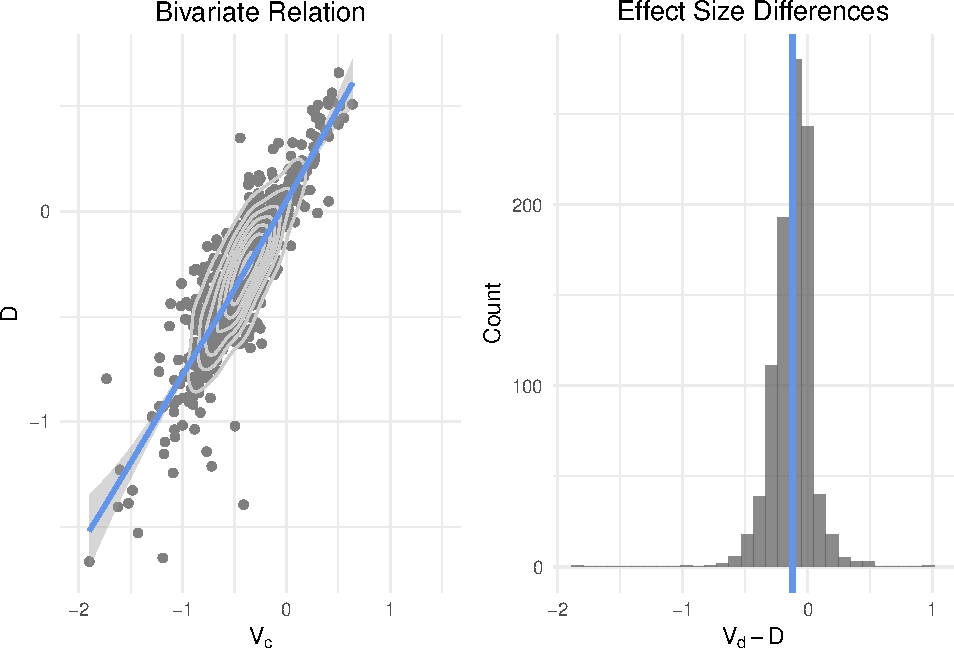
\includegraphics{anderson_ncme18_files/figure-latex/unnamed-chunk-1-1.pdf}
\caption{\label{fig:unnamed-chunk-1}Differences in Cohen's D and V estimated
with continuous data}
\end{figure}

\newpage

\hypertarget{references}{%
\section{References}\label{references}}

\begingroup\setlength{\parindent}{-0.5in}\setlength{\leftskip}{0.25in}

\hypertarget{refs}{}
\leavevmode\hypertarget{ref-esvis}{}%
Anderson, D. (2018). \emph{Esvis: Visualization and estimation of effect
sizes}. Retrieved from \url{https://github.com/DJAnderson07/esvis}

\leavevmode\hypertarget{ref-bowen99}{}%
Bowen, N. K., \& Bowen, G. L. (1999). Effects of crime and violence in
neighborhoods and schools on the school behavior and performance of
adolescents. \emph{Journal of Adolescent Research}, \emph{14}(3),
319--342.

\leavevmode\hypertarget{ref-ca17b}{}%
California Department of Education. (2017). \emph{Public schools and
districts files}. Retrieved March 24, 2018, from
\url{https://www.cde.ca.gov/ds/si/ds/pubschls.asp}

\leavevmode\hypertarget{ref-leaflet}{}%
Cheng, J., Karambelkar, B., \& Xie, Y. (2017). \emph{Leaflet: Create
interactive web maps with the javascript 'leaflet' library}. Retrieved
from \url{https://CRAN.R-project.org/package=leaflet}

\leavevmode\hypertarget{ref-dawes16}{}%
Dawes, S. S., Vidiasova, L., \& Parkhimovich, O. (2016). Planning and
designing open government data programs: An ecosystem approach.
\emph{Government Information Quarterly}, \emph{33}(1), 15--27.

\leavevmode\hypertarget{ref-gonzales96}{}%
Gonzales, N. A., Cauce, A. M., Friedman, R. J., \& Mason, C. A. (1996).
Family, peer, and neighborhood influences on academic achievement among
african-american adolescents: One-year prospective effects.
\emph{American Journal of Community Psychology}, \emph{24}(3), 365.

\leavevmode\hypertarget{ref-google}{}%
Google. (2018, March 15). \emph{Google maps api}. Retrieved March 24,
2018, from
\url{https://developers.google.com/maps/documentation/geocoding/start}

\leavevmode\hypertarget{ref-gregory10}{}%
Gregory, A., Skiba, R. J., \& Noguera, P. A. (2010). The achievement gap
and the discipline gap: Two sides of the same coin? \emph{Educational
Researcher}, \emph{39}(1), 59--68.

\leavevmode\hypertarget{ref-hanushek09}{}%
Hanushek, E. A., Kain, J. F., \& Rivkin, S. G. (2009). New evidence
about brown v. Board of education: The complex effects of school racial
composition on achievement. \emph{Journal of Labor Economics},
\emph{27}(3), 349--383.

\leavevmode\hypertarget{ref-ho08}{}%
Ho, A. D. (2008). The problem with ``proficiency'': Limitations of
statistics and policy under no child left behind. \emph{Educational
Researcher}, \emph{37}(6), 351--360.

\leavevmode\hypertarget{ref-ho09}{}%
Ho, A. D. (2009). A nonparametric framework for comparing trends and
gaps across tests. \emph{Journal of Educational and Behavioral
Statistics}, \emph{34}(2), 201--228.

\leavevmode\hypertarget{ref-ho12}{}%
Ho, A. D., \& Reardon, S. F. (2012). Estimating achievement gaps from
test scores reported in ordinal ``proficiency'' categories.
\emph{Journal of Educational and Behavioral Statistics}, \emph{37}(4),
489--517.

\leavevmode\hypertarget{ref-holland02}{}%
Holland, P. W. (2002). Two measures of change in the gaps between the
cdfs of test-score distributions. \emph{Journal of Educational and
Behavioral Statistics}, \emph{27}(1), 3--17.

\leavevmode\hypertarget{ref-ies16}{}%
Institute of Education Sciences. (2016, October). \emph{IES policy
regarding public access to research}. Retrieved March 24, 2018, from
\url{https://ies.ed.gov/funding/researchaccess.asp}

\leavevmode\hypertarget{ref-nih_16}{}%
Kittrie, E., \& Chattopadhyay, S. (2016). \emph{NIH makes data sharing
repositories publically viewable on healtdata.gov}. Retrieved March 22,
2018, from \url{https://datascience.nih.gov/Blog_HealthData.gov}

\leavevmode\hypertarget{ref-lee09}{}%
Lee, M., \& Madyun, N. (2009). The impact of neighborhood disadvantage
on the black--white achievement gap. \emph{Journal of Education for
Students Placed at Risk}, \emph{14}(2), 148--169.

\leavevmode\hypertarget{ref-mccoy13}{}%
McCoy, D. C., Roy, A. L., \& Sirkman, G. M. (2013). Neighborhood crime
and school climate as predictors of elementary school academic quality:
A cross-lagged panel analysis. \emph{American Journal of Community
Psychology}, \emph{52}(1-2), 128--140.

\leavevmode\hypertarget{ref-nsf16}{}%
National Science Foundation. (2016). \emph{The national science
foundation open government plan} (No. MSU-CSE-06-2).

\leavevmode\hypertarget{ref-nclb02}{}%
No Child Left Behind. (2002). Act of 2001, 20 usca 6301 et seq.

\leavevmode\hypertarget{ref-or17a}{}%
Oregon Department of Education. (2017a). \emph{Student assessment}.
Retrieved March 24, 2018, from
\url{http://www.oregon.gov/ode/educator-resources/assessment/Pages/Assessment-Group-Reports.aspx}

\leavevmode\hypertarget{ref-or17b}{}%
Oregon Department of Education. (2017b). Retrieved March 24, 2018, from
\url{http://www.ode.state.or.us/pubs/labels/SchoolMail.xls}

\leavevmode\hypertarget{ref-r}{}%
R Core Team. (2017). \emph{R: A language and environment for statistical
computing}. Vienna, Austria: R Foundation for Statistical Computing.
Retrieved from \url{https://www.R-project.org/}

\leavevmode\hypertarget{ref-reardon15}{}%
Reardon, S. F., \& Ho, A. D. (2015). Practical issues in estimating
achievement gaps from coarsened data. \emph{Journal of Educational and
Behavioral Statistics}, \emph{40}(2), 158--189.

\leavevmode\hypertarget{ref-sieber15}{}%
Sieber, R. E., \& Johnson, P. A. (2015). Civic open data at a
crossroads: Dominant models and current challenges. \emph{Government
Information Quarterly}, \emph{32}(3), 308--315.

\leavevmode\hypertarget{ref-sirin05}{}%
Sirin, S. R. (2005). Socioeconomic status and academic achievement: A
meta-analytic review of research. \emph{Review of Educational Research},
\emph{75}(3), 417--453.

\leavevmode\hypertarget{ref-ca17a}{}%
Studnet Performance, C. A. of, \& Progress. (2017). \emph{Test results
for english language arts/literacy and mathematics}. Retrieved March 24,
2018, from \url{https://caaspp.cde.ca.gov/sb2017/ResearchFileList}

\leavevmode\hypertarget{ref-tidycensus}{}%
Walker, K. (2018). \emph{Tidycensus: Load us census boundary and
attribute data as 'tidyverse' and 'sf'-ready data frames}. Retrieved
from \url{https://github.com/walkerke/tidycensus}

\leavevmode\hypertarget{ref-tidyverse}{}%
Wickham, H. (2017). \emph{Tidyverse: Easily install and load the
'tidyverse'}. Retrieved from
\url{https://CRAN.R-project.org/package=tidyverse}

\leavevmode\hypertarget{ref-zuiderwijk14}{}%
Zuiderwijk, A., \& Janssen, M. (2014). Open data policies, their
implementation and impact: A framework for comparison. \emph{Government
Information Quarterly}, \emph{31}(1), 17--29.

\endgroup






\end{document}
